% 3.4.3 Conexión con WhatsApp Cloud API (T6). Sin tokens ni identificadores de Meta.

\subsubsection{Conexión con WhatsApp Cloud API}

La conexión sigue los mecanismos del diseño (Tabla~\ref{tab:ob2_mecanismos}). La Tabla~\ref{tab:ob3_meta} resume la configuración, y la Figura~\ref{fig:ob3_meta}, el webhook verificado.

\begingroup
\fontsize{9}{11}\selectfont
\renewcommand{\arraystretch}{1.2}
\setlength{\LTpre}{0pt}\setlength{\LTpost}{6pt}
\setlength{\tabcolsep}{4pt}
\begin{xltabular}{\linewidth}{|>{\raggedright\arraybackslash}p{3.4cm}|>{\raggedright\arraybackslash}X|}
\caption{Configuración de WhatsApp Cloud API}
\label{tab:ob3_meta} \\
\hline
\textbf{Elemento} & \textbf{Configuración} \\ \hline
\endfirsthead
\hline
\textbf{Elemento} & \textbf{Configuración} \\ \hline
\endhead
Cuenta y aplicación & Cuenta de desarrollador de Meta y aplicación con el producto WhatsApp, a nombre del centro y sin verificación de la empresa \\ \hline
Número & De prueba de Meta en desarrollo; chip prepago dedicado solo al agente en producción. Recepción conserva su número \\ \hline
Webhook & Subdominio \textit{bot} por HTTPS, verificado por Meta y suscrito a los mensajes; la firma de cada mensaje se valida con el secreto de la aplicación \\ \hline
Credenciales & Token permanente de un usuario del sistema, guardado solo en el servidor \\ \hline
\end{xltabular}
\endgroup

\begin{figure}[H]
\centering
\IfFileExists{img/Objetivo3/Ob3_Meta_Webhook.png}{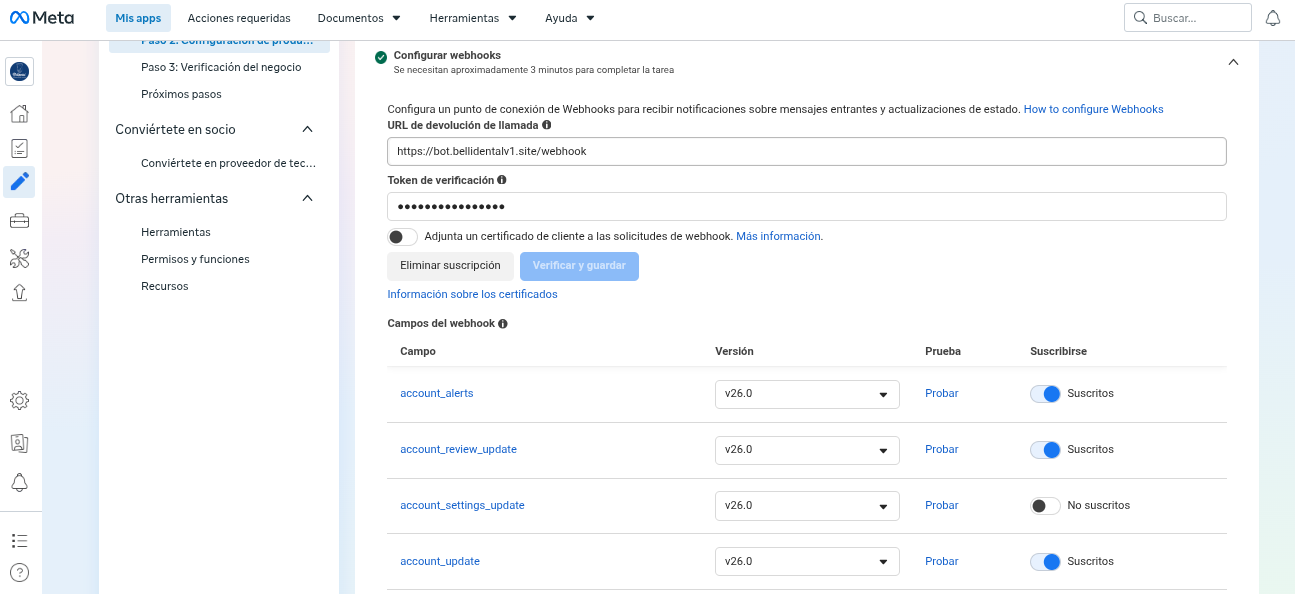
\includegraphics[width=\linewidth]{img/Objetivo3/Ob3_Meta_Webhook.png}}{\fbox{\parbox{0.9\linewidth}{\centering Pendiente: img/Objetivo3/Ob3\_Meta\_Webhook.png}}}
\caption{Webhook del agente configurado en la aplicación de Meta}
\label{fig:ob3_meta}
\end{figure}
